\documentclass[11pt,a4paper,titlepage]{article}
\usepackage[utf8]{inputenc}
\usepackage{amssymb}
\usepackage[english,polish]{babel}
\usepackage[T1]{fontenc}
\usepackage{polski}
%\usepackage[math,light]{anttor}
\usepackage[light]{anttor}
\usepackage{amsmath}
\usepackage{amsfonts}
\usepackage{graphicx}
\usepackage{sidecap}
%\usepackage{wrapfig}
\usepackage{epstopdf}
\usepackage{booktabs}
\usepackage{forloop}
\usepackage[left=3cm,right=3cm,top=3cm,bottom=3cm]{geometry}
\usepackage[framed,numbered,autolinebreaks]{mcode}
\usepackage[colorlinks=false,urlcolor=blue,citecolor=green]{hyperref}
\usepackage{fancyhdr}
\usepackage{lastpage}
\usepackage{array}
\usepackage{hhline}
\usepackage{svg}
\usepackage{multirow}
\usepackage{enumerate}%[I], numerki, [(a)]
\usepackage{float}
%\usepackage{courier}
%ustawienie poziomów wypunktowania do wyboru: $\bullet$, $\cdot$, $\diamond$, $-$, $\ast$ and $\circ$ 
\renewcommand{\labelitemi}{$\diamond$}
\renewcommand{\labelitemii}{$\bullet$}
\renewcommand{\labelitemiii}{$-$}
\renewcommand{\labelitemiv}{$\ast$}

%Figure numbering
\usepackage{chngcntr}
\counterwithin{figure}{section}
\counterwithin{equation}{section}

\newcommand*{\captionsource}[2]{%
  \caption[{#1}]{%
    #1%
    \\\hspace{\linewidth}%
    \textbf{Źródło:} #2%
  }%
}

\AtBeginDocument{

	\renewcommand{\tablename}{Tabela}

	\renewcommand{\figurename}{Rys.}
}

%tabelki
\usepackage{tabularx}
\newcolumntype{A}{>{\centering\arraybackslash}X}
\newcolumntype{B}{>{\centering\arraybackslash} m{0.4\textwidth} }


% --- < bibliografia > ---
\usepackage[
style=numeric,
sorting=none,
% Zastosuj styl wpisu bibliograficznego właściwy językowi publikacji.
language=auto,
autolang=other,
% Zapisuj datę dostępu do strony WWW w formacie RRRR-MM-DD.
urldate=iso8601,
% Nie dodawaj numerów stron, na których występuje cytowanie.
backref=false,
% Podawaj ISBN.
isbn=true,
% Nie podawaj URL-i, o ile nie jest to konieczne.
url=false,
% Ustawienia związane z polskimi normami dla bibliografii.
maxbibnames=3,
% Jeżeli używamy BibTeXa:
backend=bibtex
]{biblatex}
% --- < bibliografia > --- Koniec

\usepackage{csquotes}
\DeclareQuoteAlias{croatian}{polish} % Ponieważ `csquotes` nie posiada polskiego stylu, można skorzystać z mocno zbliżonego stylu chorwackiego.

\addbibresource{bibliografia.bib}

\pagestyle{fancy}
\fancyhf{}
\fancyhead[R]{Segway}
\fancyfoot[R]{Optymalizacja w Systemach Sterowania}
\fancyhead[L]{M. Kowalczyk i M. Podsiadło}     
\fancyfoot[L]{Strona \thepage \hspace{1pt} z\hspace{1pt} \pageref*{LastPage}}    
\renewcommand{\headrulewidth}{1pt}
\renewcommand{\footrulewidth}{1pt}

\begin{document}
\begin{titlepage}

\newcommand{\HRule}{\rule{\linewidth}{0.5mm}} % Defines a new command for the horizontal lines, change thickness here

\center % Center everything on the page
 
%----------------------------------------------------------------------------------------
%	HEADING SECTIONS
%----------------------------------------------------------------------------------------

\textsc{\LARGE Akademia Górniczo - Hutnicza im. Stanisława Staszica}\\[0.5cm]

\includegraphics[scale=0.6]{agh}\\[1cm] % Name of your university/college
\textsc{\Large Wydział Elektrotechniki, Automatyki, Informatyki i Inżynierii Biomedycznej}\\[0.5cm] % Major heading such as course name
\textsc{\large Kierunek: Automatyka i robotyka}\\[0.5cm] % Minor heading such as course title

%----------------------------------------------------------------------------------------
%	TITLE SECTION
%----------------------------------------------------------------------------------------

\HRule \\[0.4cm]
{ \huge \bfseries Optymalizacja w Systemach Sterowania\\[1cm]Segway}\\[0.4cm] % Title of your document
\HRule \\[2cm]%[3.5cm]
 


%----------------------------------------------------------------------------------------
%	DATE SECTION
%----------------------------------------------------------------------------------------

{\large czerwiec 2017}\\[1.5cm] % Date, change the \today to a set date if you want to be precise

%----------------------------------------------------------------------------------------
%	LOGO SECTION
%----------------------------------------------------------------------------------------

%
\includegraphics[height=70mm]{agh.jpg}%\\[1cm] % Include a department/university logo - this will require the graphicx package
%----------------------------------------------------------------------------------------
%	AUTHOR SECTION
%----------------------------------------------------------------------------------------

\begin{flushleft}
\Large
\emph{Wykonali:}\\
Marcin Kowalczyk\\
Maciej Podsiadło\\[1cm]

% If you don't want a supervisor, uncomment the two lines below and remove the section above
 \emph{Prowadzący:}\\
dr hab. inż. prof. AGH Adam Korytowski\\[3cm] % Your name
 
\end{flushleft}
%----------------------------------------------------------------------------------------
\end{titlepage}
\clearpage
\setcounter{page}{2}
 
\clearpage
\tableofcontents
\clearpage

\section{Wstęp}
\label{sec:wstep}

Celem pracy jest numeryczne wyznaczenie optymalnego sterowania dla zadania sterowania elektryczną deskorolką lub pojazdem typu \textit{Segway}. Składają się one z platformy i dwóch kół umieszczonych z boków. Pasażer stoi na platformie. Temat uznano za szczególnie ciekawy ze względu na stale rosnącą popularność Segwayów. Pierwszy tego typu pojazd został komercyjnie sprzedany w 2002 roku za kwotę 100 tys. amerykańskich dolarów! Dzisiaj użytkowników Segwayów możemy zobaczyć praktycznie wszędzie, zaczynając od pracowników supermarketów, a kończąc na turystach sprawnie poruszających się po najbardziej zatłoczonych ulicach miasta. Jego ogromną zaletą jest możliwość poruszania na zewnątrz, jak również wewnątrz większych budynków i hal. Obecnie trwają prace nad przystosowaniem Segwaya do transportu ludzi niepełnosprawnych. Brano pod uwagę również możliwość zdalnego transportu obiektu za pomocą tego urządzenia. W tym wypadku zamiast pasażera na platformie znajdowałby się ładunek. Efektem sterowania ma być przesunięcie urządzenia do zadanego punktu w przestrzeni jednowymiarowej (początkowo zakłada się ruch w przód i w tył) oraz dwuwymiarowej (koła mają różną prędkość obrotową). Jego położenie kątowe stabilizowane jest w niestabilnym punkcie równowagi (pionowo w górę). Trudności w sterowaniu są spowodowane nieliniowością dynamiki obiektu. Kryterium do oceny stanowić może zużycie energii, czas potrzebny do osiągnięcia pozycji lub dokładność osiągniętej pozycji po zadanym czasie. %Zaproponowane sterowanie postanowiono porównać z klasycznym podejściem, wykorzystującym regulator typu PID.

\begin{figure}[h]
	\centering
	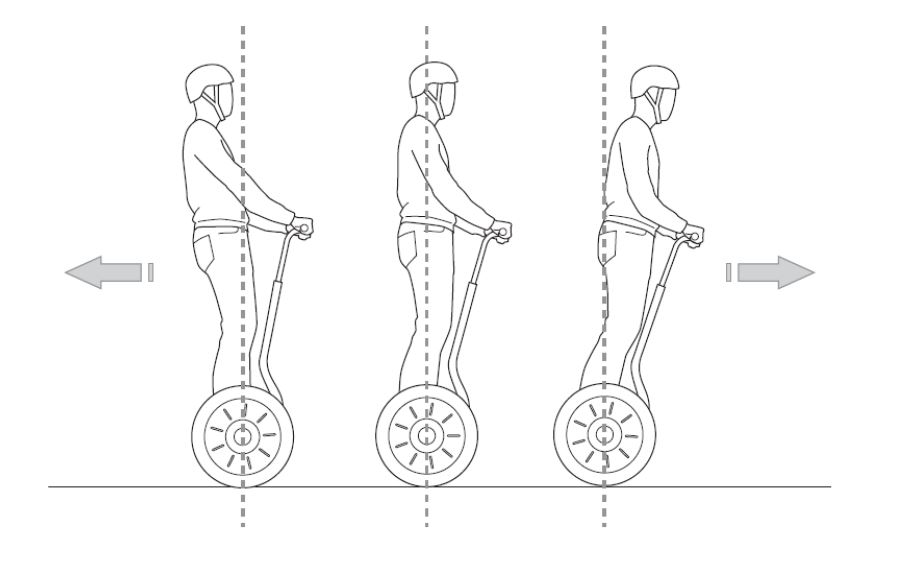
\includegraphics[width=4in]{Figures/wstep_segway.jpg}
	\captionsource{Działanie pojazdu \textit{Segway}.}{\cite{Babazadeh}}
	\label{fig:wstep_segway}
\end{figure}

Zadanie to wymaga wyznaczenia modelu matematycznego badanego obiektu oraz przetestowania jego działania. Następnie, na podstawie modelu, należy wyznaczyć optymalne sterowanie.
\section{Model matematyczny}
\label{sec:model}

W pierwszej kolejności postanowiono wyznaczyć model matematyczny obiektu sterowania. Dla tego modelu wyznaczane będzie optymalne sterowanie. Podstawową pracą z której korzystano do tego zadania jest \cite{Babazadeh}. Założono, że napęd stanowią silniki prądu stałego. Model takiego silnika w postaci równań stanu można przedstawić w następujący sposób:
\begin{equation}
\dot{x}=
\begin{bmatrix}
	-\frac{R}{L} & -\frac{k_e}{L} \\
	\frac{k_m}{I_r} & -\frac{k_e}{I_r}
\end{bmatrix}
x+
\begin{bmatrix}
	\frac{1}{L} & 0 \\
	0 & -\frac{1}{I_r}
\end{bmatrix}
u
\label{eq:dc_model_x}
\end{equation}
\begin{equation}
y=
\begin{bmatrix}
	0 & 1
\end{bmatrix}
x
\label{eq:dc_model_y}
\end{equation}
\noindent Gdzie:\newline
\(x=
\begin{bmatrix}
	i \\
	\omega
\end{bmatrix}\) jest wektorem zmiennych stanów.\newline
\(i\) jest prądem silnika.\newline
\(\omega\) jest prędkością obrotową.\newline
\(u=
\begin{bmatrix}
	V \\
	\tau
\end{bmatrix}\) jest wektorem wejść modelu.\newline
\(V\) jest napięciem podawanym na silnik.\newline
\(\tau\) jest momentem obciążenia mechanicznego.\newline
\(I_r\) jest momentem bezwładności przeniesionym na wał silnika.\newline
\(L\) jest induktancją.\newline
\(R\) jest rezystancją.\newline
\(k_e\) jest stałą elektromotoryczną.\newline
\(k_r\) jest stałą momentu silnika.

\paragraph*{}
Na rysunku \ref{fig:model_kola} przedstawiono rozkłady sił działających na koła omawianego pojazdu.

\begin{figure}[h]
	\centering
	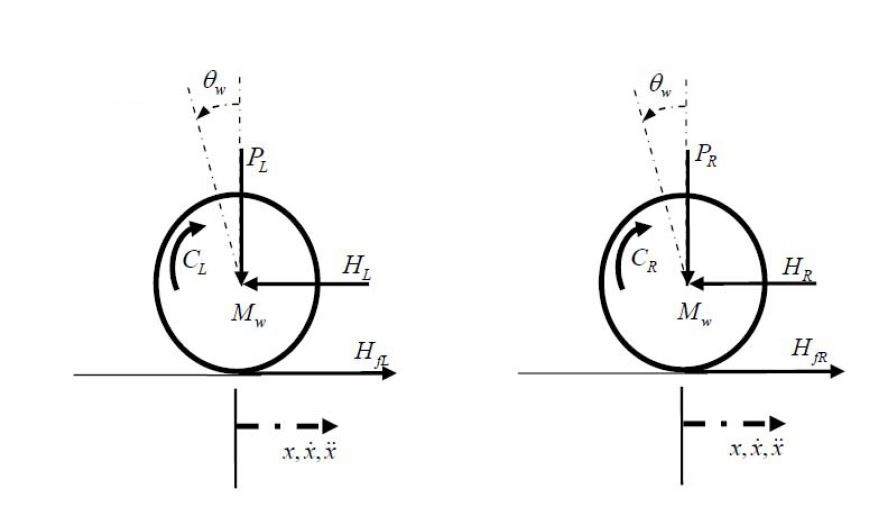
\includegraphics[width=4in]{Figures/model_kola.jpg}
	\captionsource{Siły działające na lewe i prawe koło pojazdu.}{\cite{Babazadeh}}
	\label{fig:model_kola}
\end{figure}

%TODO MK:Dodać wyprowadzenie dynamiki obiektu.

Z drugiego prawa dynamiki Newtona otrzymuje się:
\begin{equation}
\sum F_x=Ma
\end{equation}
\begin{equation}
M_w\ddot x=H_{fR}-H_R
\label{eq:newton_x}
\end{equation}
Z drugiej zasady dynamiki Newtona dla ruchu obrotowego otrzymuje się:
\begin{equation}
\sum M_o=I\alpha
\end{equation}
\begin{equation}
I_w\ddot \theta_w=C_R-H_{fR}r
\label{eq:newton_w}
\end{equation}
Moment silnika DC wynosi:
\begin{equation}
\tau_m=I_R\dot \omega+\tau_a
\label{eq:tau_m}
\end{equation}
Moment przyłożony do kół wynosi:
\begin{equation}
C=I_R\dot \omega=-\frac{k_mk_e}{R}\dot \theta_w+\frac{k_m}{R}V_a
\label{eq:C}
\end{equation}
Równanie \eqref{eq:newton_w} można więc zapisać następująco:
\begin{equation}
I_w\ddot \theta_w=-\frac{k_mk_e}{R}\dot \theta_w+\frac{k_m}{R}V_a-H_{fR}r
\end{equation}
Stąd:
\begin{equation}
H_{fR}=-\frac{k_mk_e}{Rr}\dot \theta_w+\frac{k_m}{Rr}V_a-\frac{I_w}{r}\ddot \theta_w
\label{eq:h_fr}
\end{equation}
Podstawiając \eqref{eq:h_fr} do \eqref{eq:newton_x} otrzymuje się równania dla odpowiednio prawego i lewego koła:
\begin{equation}
M_w\ddot x=-\frac{k_mk_e}{Rr}\dot \theta_w+\frac{k_m}{Rr}V_a-\frac{I_w}{r}\ddot \theta_w-H_R
\label{eq:prawe_w}
\end{equation}
\begin{equation}
M_w\ddot x=-\frac{k_mk_e}{Rr}\dot \theta_w+\frac{k_m}{Rr}V_a-\frac{I_w}{r}\ddot \theta_w-H_L
\label{eq:lewe_w}
\end{equation}
Zakłada się, że nie występuje efekt poślizgu:
\begin{equation}
\ddot \theta_w=\frac{\ddot x}{r}
\label{eq:dd_theta_w}
\end{equation}
\begin{equation}
\dot \theta_w=\frac{\dot x}{r}
\label{eq:d_theta_w}
\end{equation}
Powyższe zależności uwzględnia się we wzorach \eqref{eq:prawe_w} i \eqref{eq:lewe_w}:
\begin{equation}
M_w\ddot x=-\frac{k_mk_e}{Rr^2}\dot x+\frac{k_m}{Rr}V_a-\frac{I_w}{r^2}\ddot x-H_R
\label{eq:prawe_x}
\end{equation}
\begin{equation}
M_w\ddot x=-\frac{k_mk_e}{Rr^2}\dot x+\frac{k_m}{Rr}V_a-\frac{I_w}{r^2}\ddot x-H_L
\label{eq:lewe_x}
\end{equation}
\begin{equation}
2(M_w+\frac{I_w}{r^2})\ddot x=-\frac{2k_mk_e}{Rr^2}\dot x+\frac{2k_m}{Rr}V_a-(H_R+H_L)
\label{eq:total_x}
\end{equation}

\paragraph*{}
Przeanalizować należy również siły działające na użytkownika i drążek sterowania. Zostały one potraktowane jako elementy sztywne. Przedstawiono je na rysunku \ref{fig:model_raczka}.

\begin{figure}[H]
	\centering
	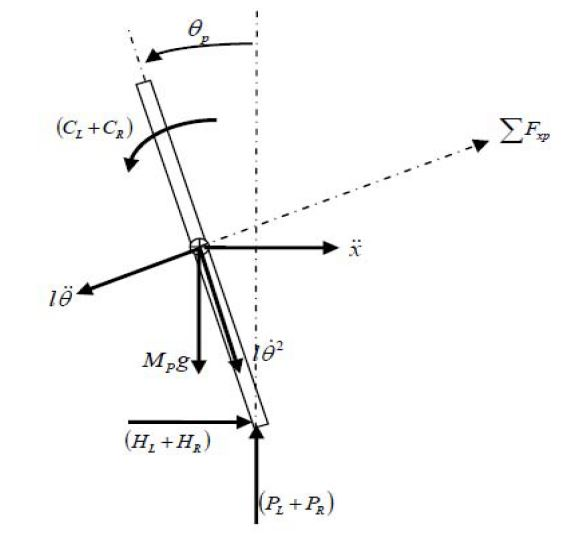
\includegraphics[width=4in]{Figures/model_raczka.jpg}
	\captionsource{Siły działające na pasażera i drążek sterowania.}{\cite{Babazadeh}}
	\label{fig:model_raczka}
\end{figure}

Z drugiej zasadny dynamiki Newtona dla osi x otrzymuje się:
\begin{equation}
\sum F_x=M_p\ddot x
\end{equation}
\begin{equation}
(H_L+H_R)=M_pl\ddot \theta_p\cos \theta_p-M_pl\dot \theta_p^2\sin \theta_p+M_p\ddot x
\label{eq:sum_H}
\end{equation}
Suma sił przyłożonych do drążka i pasażera wynosi:
\begin{equation}
\sum F_{xp}=M_p\ddot x\cos \theta_p
\end{equation}
\begin{equation}
(H_L+H_R)\cos \theta_p+(P_L+P_R)\sin \theta_p-M_pl\ddot \theta_p-M_pg \sin \theta_p=M_p \ddot x \cos \theta_p
\label{eq:sum_forces_rid_hand}
\end{equation}
Moment obrotowy działający na pasażera i drążek względem środka ich masy wynosi:
\begin{equation}
\sum M_o=I\alpha
\end{equation}
\begin{equation}
-(H_L+H_R)l\cos \theta_p+(P_L+P_R)l\sin \theta_p+(C_L+C_R)=I_p\ddot \theta_p
\label{eq:moment_pas_dr}
\end{equation}
Na podstawie równań \eqref{eq:total_x}, \eqref{eq:dd_theta_w} i \eqref{eq:d_theta_w} moment działający na pasażera i drążek wynosi:
\begin{equation}
(C_L+C_R)=-\frac{2k_mk_e}{Rr}\dot x+\frac{2k_m}{R}V_a
\label{eq:sum_C}
\end{equation}
Podstawiając \eqref{eq:C} do \eqref{eq:moment_pas_dr} otrzymuje się:
\begin{equation}
-(H_L+H_R)l\cos \theta_p+(P_L+P_R)l\sin \theta_p+(-\frac{2k_mk_e}{Rr}\dot x+\frac{2k_m}{R}V_a)-I_p\ddot \theta_p
\label{eq:moment_pas_dr_C}
\end{equation}
Po podstawieniu \eqref{eq:sum_forces_rid_hand} do \eqref{eq:moment_pas_dr_C} otrzymuje się:
\begin{equation}
I_p\ddot \theta_p-\frac{2k_mk_e}{Rr}\dot x+\frac{2k_m}{R}V_a+M_pl^2\ddot \theta_p+M_pgl \sin \theta_p=-M_pl\ddot x\cos \theta_p
\end{equation}
Alby wyeliminować \((H_L+H_R)\) z modelu, równanie \eqref{eq:sum_H} podstawia się do równania \eqref{eq:total_x}:
\begin{equation}
2(M_w+\frac{I_w}{r^2})\ddot x=-\frac{2k_mk_e}{Rr^2}+\frac{2k_m}{Rr}V_a-M_pl\ddot \theta_p \cos \theta_p+M_pl\dot \theta_p^2\sin \theta_p-M_p\ddot x
\end{equation}
Na podstawie powyższych wyprowadzeń otrzymano nieliniowe równania dynamiki obiektu:
\begin{equation}
(M_pl^2+I_p)\ddot \theta_p-\frac{2k_mk_e}{Rr}\dot{x}+\frac{2k_m}{R}V_a+M_pgl\sin \theta_p=-M_pl\ddot x\cos \theta_p
\end{equation}
\begin{equation}
\frac{2k_m}{Rr}V_a=(2M_w+\frac{2I_w}{r^2}+M_p)\ddot x+\frac{2k_mk_e}{Rr^2}\dot x+M_pl\ddot \theta_p\cos \theta_p-M_pl\dot \theta_p^2\sin \theta_p
\end{equation}
Równania te przekształcono do postaci nieliniowych równań stanu:
\begin{equation}
\begin{aligned}
\dot x_1 &= x_2\\
\dot x_2 &= -\frac{a_8}{a_7}x_2-\frac{a_9}{a_7}\cdot \frac{(\frac{a_5a_6}{a_7}\sin x_3-a_3)u-(\frac{a_5a_8}{a_7}\sin x_3+a_2)x_2-a_4\sin x_3}{a_1+\frac{a_5a_9}{a_7}\cos x_3\sin x_3}\cos x_3+\frac{a_6}{a_7}u\\
\dot x_3 &= x_4\\
\dot x_4 &= \frac{(\frac{a_5a_6}{a_7}\sin x_3 -a_3)u-(\frac{a_5a_8}{a_7}\sin x_3+a_2)x_2-a_4\sin x_3}{a_1+\frac{a_5a_9}{a_7}\cos x_3\sin x_3}
\end{aligned}
\label{eq:nonlinear_ss}
\end{equation}

\paragraph*{}
Opisany powyżej model zaimplementowano w programie \textit{MATLAB}. Został on przetestowany poprzez zadanie takich warunków w których można łatwo przewidzieć zachowanie rzeczywistego obiektu, np. niewielkie odchylenie od niestabilnego punktu równowagi (obiekt ustawiony pionowo do góry). Odpowiedź modelu dla tej sytuacji przedstawiono na rysunku \ref{fig:wychylenie_test}. W tym wypadku odpowiedź obiektu przypomina wahadło fizyczne. Na rysunku \ref{fig:polozenie_test} pokazano jak zmienia się położenie pojazdu w opisywanej sytuacji. Przebiegi czasowe zmiennych stanu zgadzają się z przewidywanym zachowaniem realnego urządzenia (nie biorąc pod uwagę uderzenia w ziemię).

\begin{figure}[h]
	\centering
	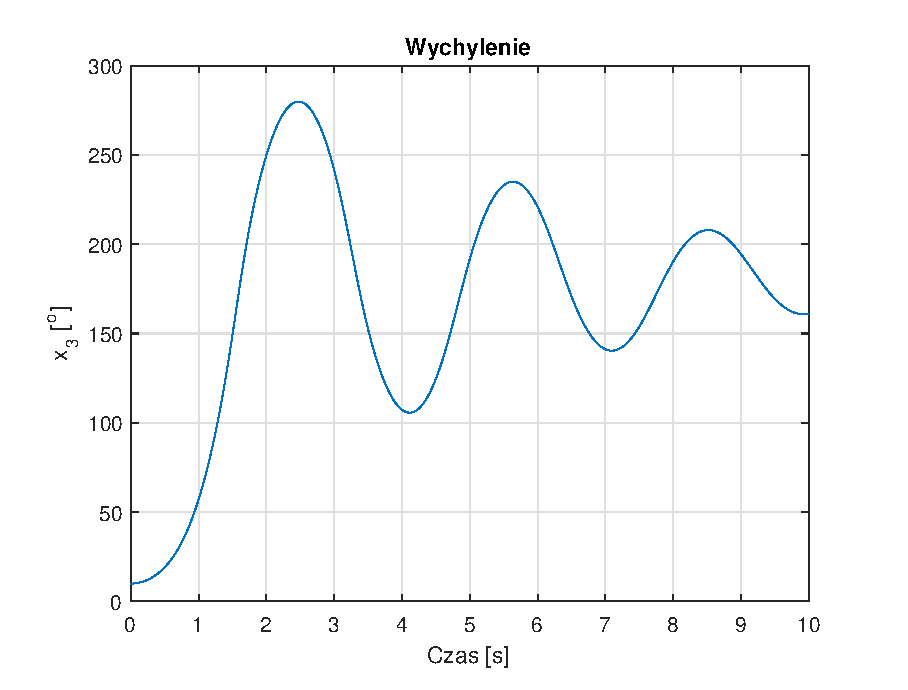
\includegraphics[width=4in]{Figures/wychylenie_test.eps}
	\caption{Wychylenie zmiennej \(x_3\) (kąta) z niestabilnego punktu równowagi.}
	\label{fig:wychylenie_test}
\end{figure}

\begin{figure}[H]
	\centering
	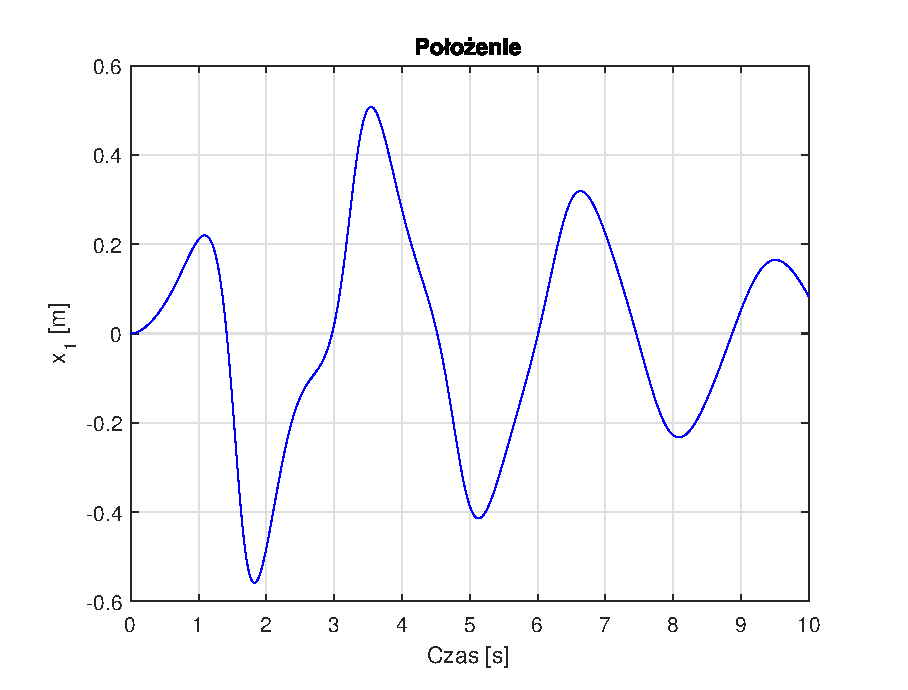
\includegraphics[width=4in]{Figures/polozenie_test.eps}
	\caption{Przebieg zmiennej \(x_1\) (położenia).}
	\label{fig:polozenie_test}
\end{figure}

Postanowiono również porównać zaimplementowaną metodę Rungego-Kutty 4-go rzędu z wbudowaną funkcją \textit{ode45}. Porównanie to dla częstotliwości próbkowania równej 1 kHz przedstawiono na rysunku \ref{fig:wychylenie_1khz}. Natomiast na rysunku \ref{fig:wychylenie_10khz} pokazano to samo porównanie dla częstotliwości próbkowania równej 10 kHz. Różnice pomiędzy tymi metodami są niewielkie. Otrzymane wyniki są prawie takie same również dla zwiększonej częstotliwości próbkowania. Można więc stwierdzić, że częstotliwość 1 kHz jest wystarczająca, do poprawnego modelowania zachowania obiektu.

\begin{figure}[h]
	\centering
	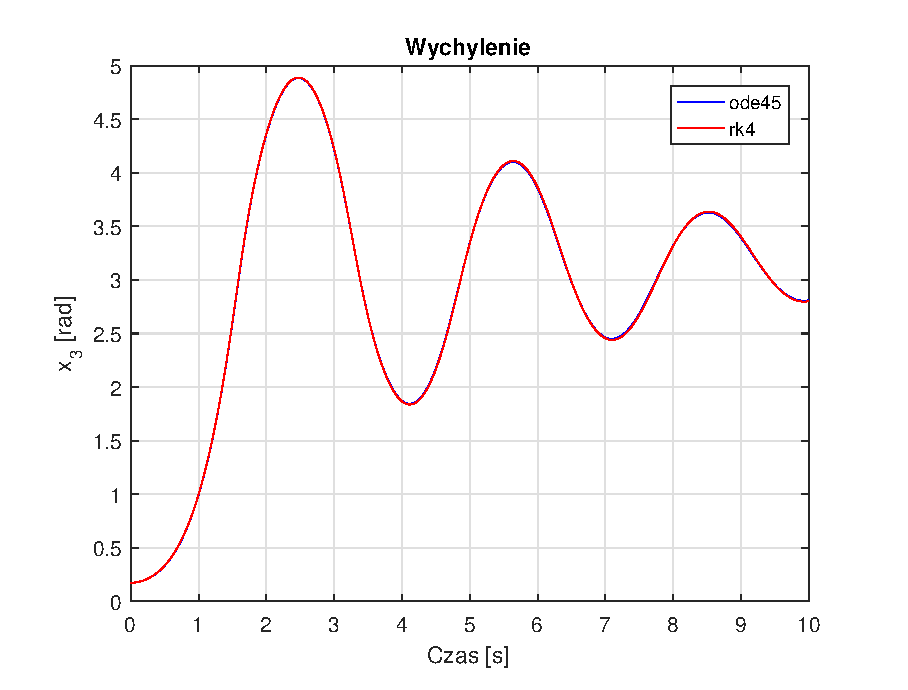
\includegraphics[width=4in]{Figures/wychylenie_1khz.eps}
	\caption{Porównanie dla częstotliwości próbkowania równej 1kHz.}
	\label{fig:wychylenie_1khz}
\end{figure}

\begin{figure}[h]
	\centering
	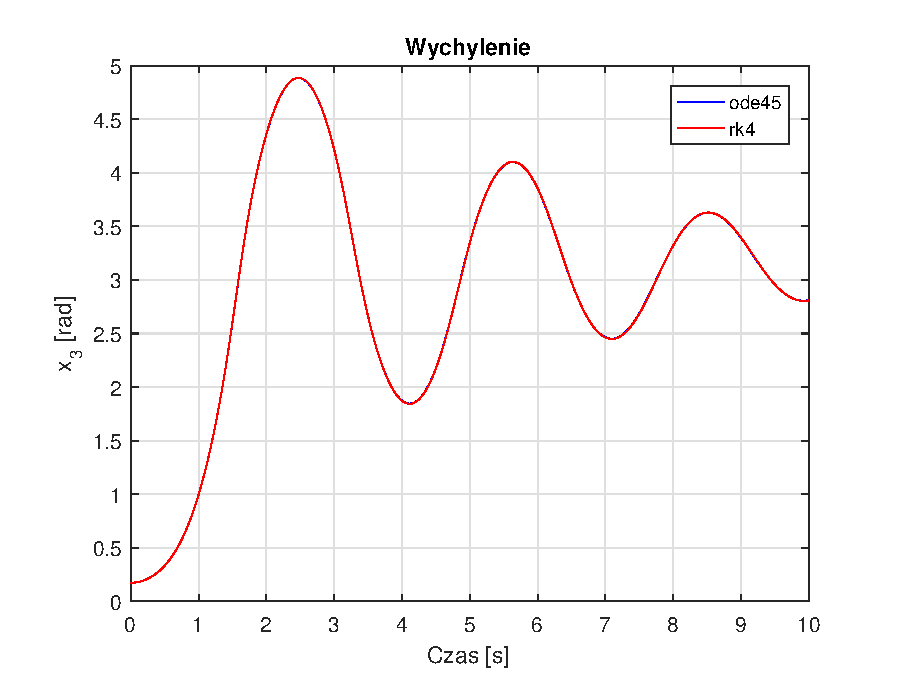
\includegraphics[width=4in]{Figures/wychylenie_10khz.eps}
	\caption{Porównanie dla częstotliwości próbkowania równej 10kHz.}
	\label{fig:wychylenie_10khz}
\end{figure}
\section{Opis używanego programu}
\label{sec:opis_uzywanego_programu}

Do wyznaczenia sterowania optymalnego wykorzystano oprogramowania \textit{Matlab}. W tym celu napisano główny skrypt, który wywoływał konieczne do wykonania zadania. W pierwszej części skryptu ustawiane są parametry symulacji, takie jak czas trwania i częstotliwość próbkowania.
\paragraph*{}
W drugiej części skryptu podawane są parametry symulowanego obiektu, takie jak:
\begin{itemize}
\item masa Segway'a
\item moment bezwładności
\item stała elektromotoryczna silnika
\item stała momentu silnika
\item maksymalne napięcie podawane na silnik
\end{itemize}
Następnie na podstawie tych parametrów wyliczone zostają współczynniki \(k_1,\dots,k_{12}\) modelu matematycznego obiektu \eqref{eq:nonlinear_ss}.
\paragraph*{}
Kolejna część programu wykorzystuje algorytm RK4 do rozwiązania numerycznego równań różniczkowych modelu. Następnie wykorzystano ten sam algorytm do rozwiązania równań sprzężonych w tył. Poprawność równań sprzężonych jest również w tej części skryptu sprawdzona.
\paragraph*{}
W ostatnim etapie skryptu uruchamiany jest algorytm optymalizacji BFGS (Broyden-Fletcher-Goldfarb-Shanno). Wyznacza on sterowanie, które minimalizuje wybrany wskaźnik jakości. Funkcja realizująca algorytm BFGS wywołuje funkcję poszukiwania na kierunku, która składa się z metody kontrakcji i ekspansji. Przebieg algorytmu optymalizacji (sterowanie w kolejnych iteracjach) jest zapisywany. Dla znalezionego sterowania optymalnego wyznaczany jest przebieg zmiennych stanu obiektu. Przebiegi zmiennych stanu dla wyznaczonego sterowania oraz samo sterowania zostają następnie pokazane na wykresach.
\section{Zasada maksimum Pontriagina}
\label{sec:zasada_max}

W celu wyznaczenia sterowania optymalnego bazowano na teorii sformułowanej przez rosyjskiego matematyka, Lewa Pontriagina, w 1956 roku. Zasada maksimum Pontriagina okazuje się mieć duże znaczenie w praktyce co czyni ją szczególnie cenną. Rozwiązywanie postawionego problemu rozpoczęto od jego matematycznego sformułowania. Dynamika pojazdu opisana jest równaniami różniczkowymi postaci:
\begin{equation}
\dot{x}(t)=f(x(t),u(t))
\end{equation}
\noindent Gdzie:\newline
$x(t)\in\textbf{R}^{4}$ oznacza stan systemu.\newline
$x_1(t)$ jest położeniem Segwaya wyrażonym w metrach.\newline
$x_2(t)$ jest prędkością liniową Segwaya wyrażoną w metrach na sekundę.\newline
$x_3(t)$ jest położeniem kątowym Segwaya wyrażonym w radianach.\newline
$x_4(t)$ jest prędkością kątową Segwaya wyrażoną w radianach na sekundę.\newline
$u(t)\in\textbf{R}$ oznacza sterowanie (napięcie podawane na silnik DC).\newline
\paragraph*{}
Punkt początkowy $x(0)=x_0$ jest ustalony. Rozwiązanie równań stanu nie zależy wprost od czasu - problem jest stacjonarny. Za zmienną decyzyjną przyjęto sterowanie, które ma postać funkcji przedziałami ciągłej. Ilość przedziałów zależy od wyboru ilości węzłów strukturalnych, która traktowana będzie jako parametr wywołania programu wyliczającego sterowanie optymalne. Wartości sterowania należą do zbioru dopuszczalnego, posiadającego kres górny oraz dolny. Założenie to uznajemy za konieczne, w przeciwnym wypadku należałoby spodziewać się, że sterowanie w kolejnych przedziałach przyjmowałoby bardzo duże wartości. Takie rozwiązanie nie miałoby fizycznego sensu. Wskaźnik jakości jest postaci:
\begin{equation}
Q(u)=q1(x(T))+\int\limits_{0}^{T}p(x_3(t))dt
\end{equation}
\noindent Gdzie:\newline
\(\int\limits_{0}^{T}p(x_3(t))dt\geq0\) wyraża karę za nadmierne odchylenie Segwaya od niestabilnego punktu równowagi.\newline
\(T\) oznacza ustaloną chwilę końcową.
\paragraph*{}
Za najbardziej interesujące rozwiązanie uznano takie, w którym T jest jak najmniejsze (przy równoczesnym braku istotnego pogorszenia wskaźnika jakości). Postanowiono zastosować metodę kontynuacyjną. \newline
Problem o tak sformułowanym wskaźniku jakości nosi nazwę Bolzy. Poprzez prosty zabieg matematyczny sprowadzono powyższe równanie do postaci Mayera. W tym celu rozszerzono przestrzeń stanu systemu o kolejną zmienną:
\begin{equation}
\begin{aligned}
x_5(t)&=\int\limits_{0}^{T}p(x_3(t))dt \\
\dot{x}_5(t)&=p(x_3(t))\\
x_5(0)&=0\\
Q(u)&=q(x(T))
\end{aligned}
\end{equation}
Korzystając z przekształconej postaci wskaźnika zapisano prehamiltonian
\begin{equation}
H(\psi(t),x(t),u(t)=\psi(t)^Tf(x(t),u(t))
\end{equation}
gdzie $\psi$ symbolizuje funkcję sprzężoną wyznaczoną z równania
\begin{equation}
\dot \psi=-\frac{\partial f}{\partial x}\psi
\end{equation}
z warunkiem końcowym
\begin{equation}
\psi(T)=-\frac{\partial q(x(T))}{\partial x(T)}
\end{equation}
Poszukiwano sterowania $u^*(t)$, które minimalizuje wskaźnik jakości. Jednocześnie trójka $x^*(t)$, $\psi^*(t)$, $u^*(t)$ maksymalizuje prehamiltonian w każdej chwili czasu $t\in[0;T]$. Rozwiązanie tak postawionego zadania zdecydowano się aproksymować funkcją schodkową ze względu na uniwersalność takiego podejścia.


\section{Sterowanie optymalne}
\label{sec:sterowanie_optymalne}

Podstawowym celem sterowania jest utrzymanie pojazdu w pozycji pionowej. Jest to niestabilny punkt równowagi. Sterowanie powinno uwzględniać ograniczenie maksymalnego wychylenia obiektu z tego położenia oraz maksymalne napięcie podawane na silnik prądu stałego. Oprócz tego wymaga się, żeby pojazd przemieścił się o zadaną odległość przy jak najmniejszym zużyciu energii. Wybrano więc następujący wskaźnik jakości sterowania:
\begin{equation}
Q=x^T(T)x(T)
\end{equation}
\noindent Gdzie:\newline
\(x\) jest stanem obiektu.\newline
\(T\) jest horyzontem czasowym.

\paragraph*{}
Należy wziąć pod uwagę również ograniczenia:
\begin{equation}
|u(t)|< u_{max}
\label{eq:u_max}
\end{equation}
\begin{equation}
|x_3(t)|< \phi_{max}
\label{eq:phi_max}
\end{equation}
\noindent Gdzie:\newline
\(u\) jest wejściem obiektu (napięciem podawanym na silnik).\newline
\(u_{max}\) jest maksymalnym napięciem, które można podać na silnik.\newline
\(\phi_{max}\) jest maksymalnym wychyleniem pojazdu z położenia pionowego.

\paragraph*{}
Ograniczenie \eqref{eq:u_max} odnosi się do fizycznego ograniczenia napięciem akumulatora urządzenia. Nie jest możliwe podanie większego napięcia. Ograniczenie \eqref{eq:phi_max} ma na celu zabezpieczenie pojazdu przed upadkiem oraz zrzuceniem transportowanego obiektu. Nierówność \eqref{eq:phi_max} została uwzględniona w zadaniu za pomocą funkcji kary. Zadanie więc zostało zmodyfikowane do następującej postaci:
\begin{equation}
\begin{aligned}
\dot x_1 &=x_2\\
\dot x_2 &=k_1x_2+k_2\frac{L}{M}\cos x_3+k_3x_4^2\sin x_3+k_4u\\
\dot x_3 &=x_4\\
\dot x_4 &=\frac{L}{M}\\
\dot x_5 &=f_5\\
Q &=x^T(T)x(T)
\end{aligned}
\label{eq:ss_penalty}
\end{equation}
\noindent Gdzie:
\begin{equation}
\begin{aligned}
L &=(k_5\cos x_3+k_6)u+(k_7\cos x_3+k_8)x_2+k_9\sin x_3+k_{10}x_4^2\sin x_3\cos x_3\\
M &=k_{11}+k_{12}\cos ^2x_3\\
f_5 &=
	\begin{cases}
	\frac{K(x_3-\phi_{max})^2}{2}, & \text{kiedy } \phi_{max}\leqslant x_3\\
	0, & \text{kiedy } -\phi_{max}<x_3<\phi_{max}\\
	\frac{K(\phi_{max}+x_3)^2}{2}, & \text{kiedy } x_3\leqslant -\phi_{max}
	\end{cases}
\end{aligned}
\end{equation}
Dla zadania opisanego równaniami \eqref{eq:ss_penalty} wyznaczono równania sprzężone:
\begin{equation}
\dot \psi=-\frac{\partial f}{\partial x}\psi
\end{equation}
\noindent Gdzie:\newline
\(\psi\) jest wektorem funkcji sprzężonych \([\psi_1, \psi_2, \psi_3, \psi_4, \psi_5]^T\).\newline
\(f\) jest prawymi stronami układu równań stanu \eqref{eq:ss_penalty}.
\begin{equation}
\frac{\partial f}{\partial x}=\begin{bmatrix}
0 & 0 & 0 & 0 & 0\\
1 & k_2\cos(x_3)\frac{\partial S}{\partial x_2}+k_1 & 0 & \frac{\partial S}{\partial x_2} & 0\\
0 & k_3x_4^2\cos x_3+k_2\frac{\partial S}{\partial x_3}\cos x_3-k_2S\sin x_3 & 0 & \frac{\partial S}{\partial x_3} & \frac{f_5}{x_3}\\
0 & 2k_3x_4\sin x_3+k_2\frac{\partial S}{x_4}\cos x_3 & 1 & \frac{\partial S}{\partial x_4} & 0\\
0 & 0 & 0 & 0 & 0
\end{bmatrix}
\end{equation}
\noindent Gdzie:\newline
\(S=\frac{L}{M}\) jest funkcją wprowadzoną w celu uproszczenia obliczeń.
\begin{equation}
\frac{\partial f_5}{\partial x_3}=
	\begin{cases}
	K(x_3-\phi_{max}), & \text{kiedy } \phi_{max}\leqslant x_3\\
	0, & \text{kiedy } -\phi_{max}<x_3<\phi_{max}\\
	K(x_3+\phi_{max}), & \text{kiedy } x_3\leqslant -\phi_{max}
	\end{cases}
\end{equation}
Warunek końcowy równań sprzężonych jest następujący:
\begin{equation}
\psi(T)=-\frac{\partial Q}{\partial x(T)}
\end{equation}
Wiadomo, że równania sprzężone spełniają następujące równanie:
\begin{equation}
\frac{\partial Q(u,x(0)}{\partial x(0)}=-\psi(0)
\label{eq:check_psi}
\end{equation}
Postanowiono wykorzystać tę równość do sprawdzenia poprawności wyznaczonych równań sprzężonych. W tym celu konieczne było rozwiązanie równań sprzężonych do tyłu w celu wyznaczenia wartości \(-\psi(0)\). Pochodna \(\frac{\partial Q(u,x(0))}{\partial x(0)}\) została przybliżona za pomocą ilorazów różnicowych:
\begin{equation}
\frac{\partial Q(u,x(0))}{\partial x_k(0)}\approx\frac{Q(u,x_1(0),\dots, x_k(0)+\epsilon,\dots,x_n(0))}{\epsilon}
\end{equation}
\noindent Gdzie:\newline
\(\epsilon\) jest bardzo małym przyrostem (przyjmowano \(\epsilon=10^{-7}\)).
\paragraph*{}
Dla różnych przypadków testowych (różne warunki początkowe i ograniczenia) sprawdzano błąd równości \eqref{eq:check_psi}. Przykładowy błąd dla prostego zadania testowego wynosi:
\begin{equation}
\frac{\partial Q(u,x(0)}{\partial x(0)}+\psi(0)=
\begin{bmatrix}
5.14\cdot 10^{-8}\\
2.27\cdot 10^{-7}\\
1.87\cdot 10^{-5}\\
2.96\cdot 10^{-6}\\
-1.63\cdot 10^{-9}
\end{bmatrix}
\end{equation}
Błędy są bardzo małe. Na podstawie powyższego wyniku stwierdzono, że wyznaczone równania sprzężone są poprawne.\\
W trakcie numerycznego rozwiązywania wstecz równań sprzężonych wyliczano również gradient \eqref{eq:Grad}.
\begin{equation}
\begin{aligned}
&z(t) = \frac{\partial Q}{\partial u_i}=-\int\limits_{t_i}^{t_{i+1}}\frac{\partial H}{\partial u}dt&\\
&\dot{z}(t) = \frac{\partial H}{\partial u_i}, t\in [t_i,t_{i+1}]&\\
&z(t_{i+1}) = 0
\label{eq:Grad}
\end{aligned}
\end{equation}
Wymiar wektora \textit{z} jest zależny od wyboru liczby węzłów strukturalnych. Sprawdzenia poprawności wyliczonych gradientów dokonano poprzez porównanie otrzymanych wyników z ilorazem różnicowym \eqref{eq:checkGrad}.
\begin{equation}
\label{eq:checkGrad}
\frac{Q(u+\Delta u)-Q(u)}{\Delta u}
\end{equation}
Otrzymane wyniki były zgodne z dokładnością do czwartego miejsca po przecinku.
\section{Algorytm BFGS}
\label{sec:bfgs}

Sprawdziwszy poprawność funkcji wyliczającej wartość funkcji kosztu oraz jej gradient, przystąpiono do  implementacji algorytmu optymalizującego. Zdecydowano się na metodę gradientową ze względu na jej nieporównywalnie szybszą zbieżność w stosunku do metod bezgradientowych. Wybrano metodę BFGS, która należy do grupy metod kwazi-newtonowskich. Ich główną zaletą jest brak konieczności wyliczania hesjanu w każdej iteracji, co bywa często czasochłonne oraz skomplikowane numerycznie (metoda Newtona). Schemat algorytmu prezentuje się następująco:
%1. Wylosuj początkową aproksymację schodkową sterowania.\\
%2. Wylicz wartość oraz gradient funkcji kosztu.\\
%3. Sprawdź warunki stopu.\\
%4. Jeżeli to pierwsza iteracja lub nie znaleziono lepszego sterowania na kierunku to szukaj na kierunku najszybszego spadku (reset metody). Wróć do 2.\\
%5. Wyznacz nowy kierunek poszukiwań według następującej reguły:
%\begin{equation}
%\begin{aligned}
%s &=& u - uPrev\\
%r &=& dQdU - g\\
%W &=& W + \dfrac{rr^T}{s^Tr} - \dfrac{Wss^TW}{s^TWs}\\
%d &=& -W^{-1}dQdU;
%\end{aligned}
%\end{equation}
%gdzie \textit{uPrev} oraz \textit{g} to kolejno sterowanie i gradient z poprzedniej iteracji, \textit{W} oznacza przybliżony hesjan zgodnie z ideą metody BFGS, natomiast \textit{d} to wyliczony nowy kierunek poszukiwań.\\
%6. Szukaj na kierunku. Wróć do 2.
\begin{enumerate}
\item Wylosuj początkową aproksymację schodkową sterowania.
\item Wylicz wartość oraz gradient funkcji kosztu.
\item Sprawdź warunki stopu.
\item Jeżeli to pierwsza iteracja lub nie znaleziono lepszego sterowania na kierunku to szukaj na kierunku najszybszego spadku (reset metody). Wróć do 2.
\item Wyznacz nowy kierunek poszukiwań według następującej reguły:
\begin{equation}
\begin{aligned}
s &:= u - u_{prev}\\
r &:= \frac{\partial Q}{\partial u} - g\\
W &:= W + \frac{rr^T}{s^Tr} - \frac{Wss^TW}{s^TWs}\\
d &:= -W^{-1}\frac{\partial Q}{\partial u};
\end{aligned}
\end{equation}
\noindent gdzie:\newline
\(u_{prev}\) jest sterowaniem w poprzedniej iteracji\newline
\(g\) jest gradientem w poprzedniej iteracji\newline
\(W\) oznacza przybliżony hesjan zgodnie z ideą metody BFGS\newline
\(d\) jest nowym kierunkiem poszukiwań.
\item Szukaj na kierunku. Wróć do kroku 2.
\end{enumerate}

\subsection{Warunki stopu}
Algorytm powinien zakończyć swoje działanie w momencie kiedy spełniony zostanie co najmniej jeden z dwóch warunków: 
\begin{enumerate}
\item Wykorzystano maksymalną, z góry ustaloną liczbę iteracji.
\item Norma gradientu jest mniejsza od przyjętego epsilon.
\end{enumerate}
W przypadku kiedy gradient okazuje się być wystarczająco mały, można oczekiwać, że wyznaczono rozwiązanie znajdujące się blisko minimum lokalnego. Dodatkowo przy bardzo małym gradiencie próżno spodziewać się znaczącego polepszenia funkcji kosztu. Czas poświęcony na kolejne iteracje nie byłby współmierny do oczekiwanej poprawy. Jest to jedna z cech algorytmów gradientowych. W przypadku zakończenia algorytmu z powodu wyczerpania iteracji warto zwiększyć ich liczbę w kolejnym uruchomieniu programu, aby sprawdzić czy kolejne rozwiązania nie wprowadziłyby znaczącej poprawy.

\subsection{Poszukiwanie na kierunku}
Do poszukiwania lepszych rozwiązań na wyznaczonym kierunku użyto dwóch wzajemnie uzupełniających się metod - ekspansji oraz kontrakcji. Ekspansja polega na uformowaniu geometrycznego ciągu przyrostów, którego iloraz nazywany jest współczynnikiem ekspansji (większy od 1). Ekspansja kończy swoje działanie w momencie kiedy kolejne rozwiązanie jest gorsze od poprzedniego lub kiedy wyczerpie się maksymalną liczbę iteracji. W przypadku, kiedy początkowa długość kroku generuje pogorszenie wskaźnika jakości przeprowadza się kontrakcję, która polega na iteracyjny zawężaniu przedziału do momentu uzyskania pierwszej poprawy. Współczynnik kontrakcji jest mniejszy od jedynki. Ekspansja pozwala na znaczną poprawę na kierunki, natomiast kontrakcja zapewnia jakąkolwiek poprawę (o ile taka istnieje na badanym kierunku).
%TODO we wnioskach o doborze kroku i o znaczeniu poszukiwania na k. w czasie

\appendix
\nocite{*}
\printbibliography
\addcontentsline{toc}{section}{Bibliografia}
\end{document}